\documentclass{standalone}
\usepackage{tikz}
\usetikzlibrary{patterns, positioning}


\begin{document}
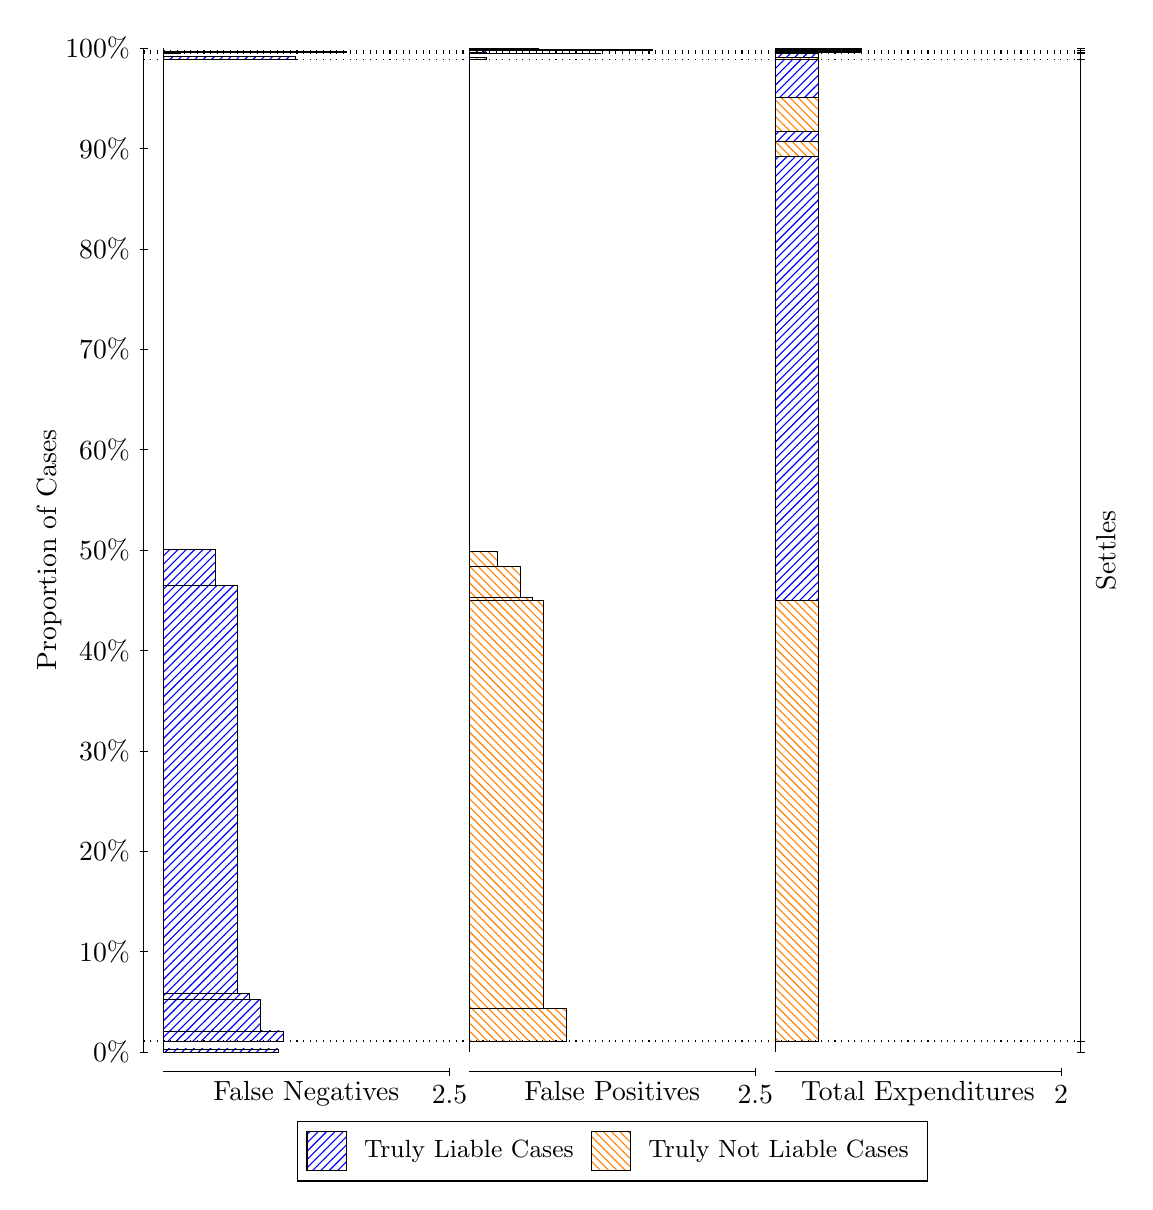
\begin{tikzpicture}
\draw[black, very thin] (1.5,1.75) -- (1.5,14.5);
\node[rotate=90, text=black, anchor=center] at (0.3, 8.125) {Proportion of Cases};
\draw[black, very thin] (1.45,1.75) -- (1.55,1.75);
\node[text=black, anchor=east] at (1.45, 1.75) {0\%};
\draw[black, very thin] (1.45,3.025) -- (1.55,3.025);
\node[text=black, anchor=east] at (1.45, 3.025) {10\%};
\draw[black, very thin] (1.45,4.3) -- (1.55,4.3);
\node[text=black, anchor=east] at (1.45, 4.3) {20\%};
\draw[black, very thin] (1.45,5.575) -- (1.55,5.575);
\node[text=black, anchor=east] at (1.45, 5.575) {30\%};
\draw[black, very thin] (1.45,6.85) -- (1.55,6.85);
\node[text=black, anchor=east] at (1.45, 6.85) {40\%};
\draw[black, very thin] (1.45,8.125) -- (1.55,8.125);
\node[text=black, anchor=east] at (1.45, 8.125) {50\%};
\draw[black, very thin] (1.45,9.4) -- (1.55,9.4);
\node[text=black, anchor=east] at (1.45, 9.4) {60\%};
\draw[black, very thin] (1.45,10.675) -- (1.55,10.675);
\node[text=black, anchor=east] at (1.45, 10.675) {70\%};
\draw[black, very thin] (1.45,11.95) -- (1.55,11.95);
\node[text=black, anchor=east] at (1.45, 11.95) {80\%};
\draw[black, very thin] (1.45,13.225) -- (1.55,13.225);
\node[text=black, anchor=east] at (1.45, 13.225) {90\%};
\draw[black, very thin] (1.45,14.5) -- (1.55,14.5);
\node[text=black, anchor=east] at (1.45, 14.5) {100\%};

\draw[black, very thin] (13.4,1.75) -- (13.4,14.5);
\draw[black, very thin] (13.35,1.75) -- (13.45,1.75);
\node[anchor=west] at (13.35, 1.75) {};
\draw[black, very thin] (13.35,1.8893) -- (13.45,1.8893);
\node[anchor=west] at (13.35, 1.8893) {};
\draw[black, very thin] (13.35,14.354) -- (13.45,14.354);
\node[anchor=west] at (13.35, 14.354) {};
\draw[black, very thin] (13.35,14.428) -- (13.45,14.428);
\node[anchor=west] at (13.35, 14.428) {};
\draw[black, very thin] (13.35,14.45) -- (13.45,14.45);
\node[anchor=west] at (13.35, 14.45) {};
\draw[black, very thin] (13.35,14.472) -- (13.45,14.472);
\node[anchor=west] at (13.35, 14.472) {};
\draw[black, very thin] (13.35,14.5) -- (13.45,14.5);
\node[anchor=west] at (13.35, 14.5) {};

\draw[black, very thin, pattern color=blue, pattern=north east lines] (1.75,1.75) rectangle (3.2033,1.7882);
\draw[black, very thin, pattern color=orange, pattern=north west lines] (1.75,1.7882) rectangle (1.75,1.8893);
\draw[black, very thin, pattern color=blue, pattern=north east lines] (1.75,1.8893) rectangle (3.276,2.0174);
\draw[black, very thin, pattern color=blue, pattern=north east lines] (1.75,2.0174) rectangle (2.9853,2.4158);
\draw[black, very thin, pattern color=blue, pattern=north east lines] (1.75,2.4158) rectangle (2.84,2.493);
\draw[black, very thin, pattern color=blue, pattern=north east lines] (1.75,2.493) rectangle (2.6947,7.6727);
\draw[black, very thin, pattern color=blue, pattern=north east lines] (1.75,7.6727) rectangle (2.404,8.1353);
\draw[black, very thin, pattern color=orange, pattern=north west lines] (1.75,8.1353) rectangle (1.75,14.354);
\draw[black, very thin, pattern color=blue, pattern=north east lines] (1.75,14.354) rectangle (3.4213,14.396);
\draw[black, very thin, pattern color=orange, pattern=north west lines] (1.75,14.396) rectangle (1.75,14.428);
\draw[black, very thin, pattern color=blue, pattern=north east lines] (1.75,14.428) rectangle (1.968,14.445);
\draw[black, very thin, pattern color=orange, pattern=north west lines] (1.75,14.445) rectangle (1.75,14.45);
\draw[black, very thin, pattern color=blue, pattern=north east lines] (1.75,14.45) rectangle (4.0753,14.461);
\draw[black, very thin, pattern color=orange, pattern=north west lines] (1.75,14.461) rectangle (1.75,14.472);
\draw[black, very thin, pattern color=orange, pattern=north west lines] (1.75,14.472) rectangle (1.75,14.479);
\draw[black, very thin, pattern color=blue, pattern=north east lines] (1.75,14.479) rectangle (1.75,14.5);
\draw[black, very thin, pattern color=orange, pattern=north west lines] (5.6333,1.75) rectangle (5.6333,1.8511);
\draw[black, very thin, pattern color=blue, pattern=north east lines] (5.6333,1.8511) rectangle (5.6333,1.8893);
\draw[black, very thin, pattern color=orange, pattern=north west lines] (5.6333,1.8893) rectangle (6.8687,2.3034);
\draw[black, very thin, pattern color=orange, pattern=north west lines] (5.6333,2.3034) rectangle (6.578,7.4831);
\draw[black, very thin, pattern color=orange, pattern=north west lines] (5.6333,7.4831) rectangle (6.4327,7.5227);
\draw[black, very thin, pattern color=orange, pattern=north west lines] (5.6333,7.5227) rectangle (6.2873,7.9211);
\draw[black, very thin, pattern color=orange, pattern=north west lines] (5.6333,7.9211) rectangle (5.9967,8.1079);
\draw[black, very thin, pattern color=blue, pattern=north east lines] (5.6333,8.1079) rectangle (5.6333,14.354);
\draw[black, very thin, pattern color=orange, pattern=north west lines] (5.6333,14.354) rectangle (5.8513,14.386);
\draw[black, very thin, pattern color=blue, pattern=north east lines] (5.6333,14.386) rectangle (5.6333,14.428);
\draw[black, very thin, pattern color=orange, pattern=north west lines] (5.6333,14.428) rectangle (7.3047,14.433);
\draw[black, very thin, pattern color=blue, pattern=north east lines] (5.6333,14.433) rectangle (5.8513,14.45);
\draw[black, very thin, pattern color=orange, pattern=north west lines] (5.6333,14.45) rectangle (5.6333,14.461);
\draw[black, very thin, pattern color=blue, pattern=north east lines] (5.6333,14.461) rectangle (5.6333,14.472);
\draw[black, very thin, pattern color=orange, pattern=north west lines] (5.6333,14.472) rectangle (7.9587,14.479);
\draw[black, very thin, pattern color=blue, pattern=north east lines] (5.6333,14.479) rectangle (6.5053,14.5);
\draw[black, very thin, pattern color=orange, pattern=north west lines] (9.5167,1.75) rectangle (9.5167,1.8511);
\draw[black, very thin, pattern color=blue, pattern=north east lines] (9.5167,1.8511) rectangle (9.5167,1.8893);
\draw[black, very thin, pattern color=orange, pattern=north west lines] (9.5167,1.8893) rectangle (10.062,7.4831);
\draw[black, very thin, pattern color=blue, pattern=north east lines] (9.5167,7.4831) rectangle (10.062,13.125);
\draw[black, very thin, pattern color=orange, pattern=north west lines] (9.5167,13.125) rectangle (10.062,13.312);
\draw[black, very thin, pattern color=blue, pattern=north east lines] (9.5167,13.312) rectangle (10.062,13.44);
\draw[black, very thin, pattern color=orange, pattern=north west lines] (9.5167,13.44) rectangle (10.062,13.878);
\draw[black, very thin, pattern color=blue, pattern=north east lines] (9.5167,13.878) rectangle (10.062,14.354);
\draw[black, very thin, pattern color=orange, pattern=north west lines] (9.5167,14.354) rectangle (10.062,14.386);
\draw[black, very thin, pattern color=blue, pattern=north east lines] (9.5167,14.386) rectangle (10.062,14.428);
\draw[black, very thin, pattern color=orange, pattern=north west lines] (9.5167,14.428) rectangle (10.062,14.433);
\draw[black, very thin, pattern color=blue, pattern=north east lines] (9.5167,14.433) rectangle (10.062,14.45);
\draw[black, very thin, pattern color=orange, pattern=north west lines] (9.5167,14.45) rectangle (10.607,14.461);
\draw[black, very thin, pattern color=blue, pattern=north east lines] (9.5167,14.461) rectangle (10.607,14.472);
\draw[black, very thin, pattern color=orange, pattern=north west lines] (9.5167,14.472) rectangle (10.607,14.479);
\draw[black, very thin, pattern color=blue, pattern=north east lines] (9.5167,14.479) rectangle (10.607,14.5);
\draw[black, dotted] (1.5,1.8893) -- (13.4,1.8893);
\draw[black, dotted] (1.5,14.354) -- (13.4,14.354);
\draw[black, dotted] (1.5,14.428) -- (13.4,14.428);
\draw[black, dotted] (1.5,14.45) -- (13.4,14.45);
\draw[black, dotted] (1.5,14.472) -- (13.4,14.472);
\draw[black, very thin] (1.75,1.5) -- (5.3833,1.5);
\node[text=black, anchor=north] at (3.5667, 1.5) {False Negatives};
\draw[black, very thin] (5.3833,1.45) -- (5.3833,1.55);
\node[text=black, anchor=north] at (5.3833, 1.45) {2.5};

\draw[black, very thin] (5.6333,1.5) -- (9.2667,1.5);
\node[text=black, anchor=north] at (7.45, 1.5) {False Positives};
\draw[black, very thin] (9.2667,1.45) -- (9.2667,1.55);
\node[text=black, anchor=north] at (9.2667, 1.45) {2.5};

\draw[black, very thin] (9.5167,1.5) -- (13.15,1.5);
\node[text=black, anchor=north] at (11.333, 1.5) {Total Expenditures};
\draw[black, very thin] (13.15,1.45) -- (13.15,1.55);
\node[text=black, anchor=north] at (13.15, 1.45) {2};


\node[text=black, centered, rotate=90] at (13.72, 8.1216) {Settles};





\draw (7.449999999999999,1.5) node[draw=none] (baseCoordinate) {};
\begin{scope}[align=center]
        \matrix[scale=0.5, draw=black, below=0.5cm of baseCoordinate, nodes={draw}, column sep=0.1cm]{
            \node[rectangle, draw, minimum width=0.5cm, minimum height=0.5cm, pattern color=blue, pattern=north east lines] {}; &
            \node[draw=none, font=\small, text=black] (B) {Truly Liable Cases}; &
            \node[rectangle, draw, minimum width=0.5cm, minimum height=0.5cm, pattern color=orange, pattern=north west lines] {}; &
            \node[draw=none, font=\small, text=black] (B) {Truly Not Liable Cases}; \\
            };
\end{scope}

\end{tikzpicture}
\end{document}